\documentclass[tikz,border=3pt]{standalone}
\usepackage[utf8]{inputenc}
\usepackage[T1]{fontenc}
\usepackage{lmodern}
\renewcommand{\familydefault}{\sfdefault}
\usepackage{sansmath}\sansmath
\usepackage{chemfig}
\usepackage{pgfplots}\pgfplotsset{compat=1.18,/pgf/number format/use comma,/pgf/number format/1000 sep={.}}
\usetikzlibrary{arrows.meta,calc,positioning,decorations.pathmorphing,decorations.pathreplacing,patterns}
% paleta del sitio
\definecolor{nar}{HTML}{E8680C}\definecolor{narc}{HTML}{FFB35C}\definecolor{hielo}{HTML}{FFF3E8}
\definecolor{tinta}{HTML}{1D1D1F}\definecolor{gris}{HTML}{6E6E73}\definecolor{lila}{HTML}{7C5CF0}
\definecolor{azul}{HTML}{2F6FD6}\definecolor{menta}{HTML}{17A673}\definecolor{coral}{HTML}{E8342A}
\begin{document}
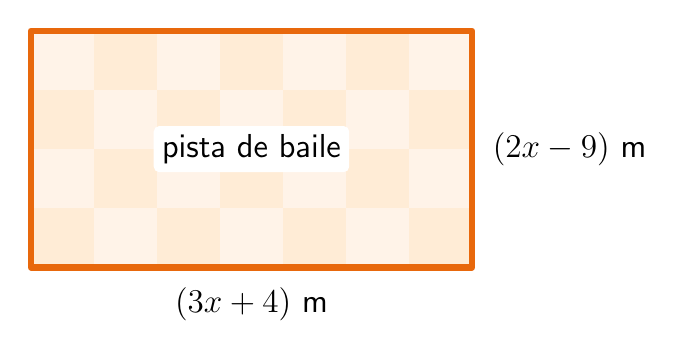
\begin{tikzpicture}[font=\large,line join=round]
\def\L{5.6}\def\H{3.0}
\fill[hielo] (0,0) rectangle (\L,\H);
\foreach \i in {0,...,6} \foreach \j in {0,...,3} {\pgfmathtruncatemacro\m{mod(\i+\j,2)}\ifnum\m=0\fill[narc!25] (\i*0.8,\j*0.75) rectangle ++(0.8,0.75);\fi}
\draw[nar,line width=2.4pt] (0,0) rectangle (\L,\H);
\node[fill=white,rounded corners=2pt,inner sep=3pt] at (\L/2,\H/2) {pista de baile};
\node[below=4pt] at (\L/2,0) {$(3x+4)$ m};
\node[right=4pt] at (\L,\H/2) {$(2x-9)$ m};
\end{tikzpicture}
\end{document}
